\hypertarget{des-uxe9lections...uxe0-la-foruxeat-des-cuxe8dres}{%
\section{Des élections...à la forêt des
Cèdres}\label{des-uxe9lections...uxe0-la-foruxeat-des-cuxe8dres}}

\emph{Jeudi 17 mai 2018}

\begin{figure}
\centering
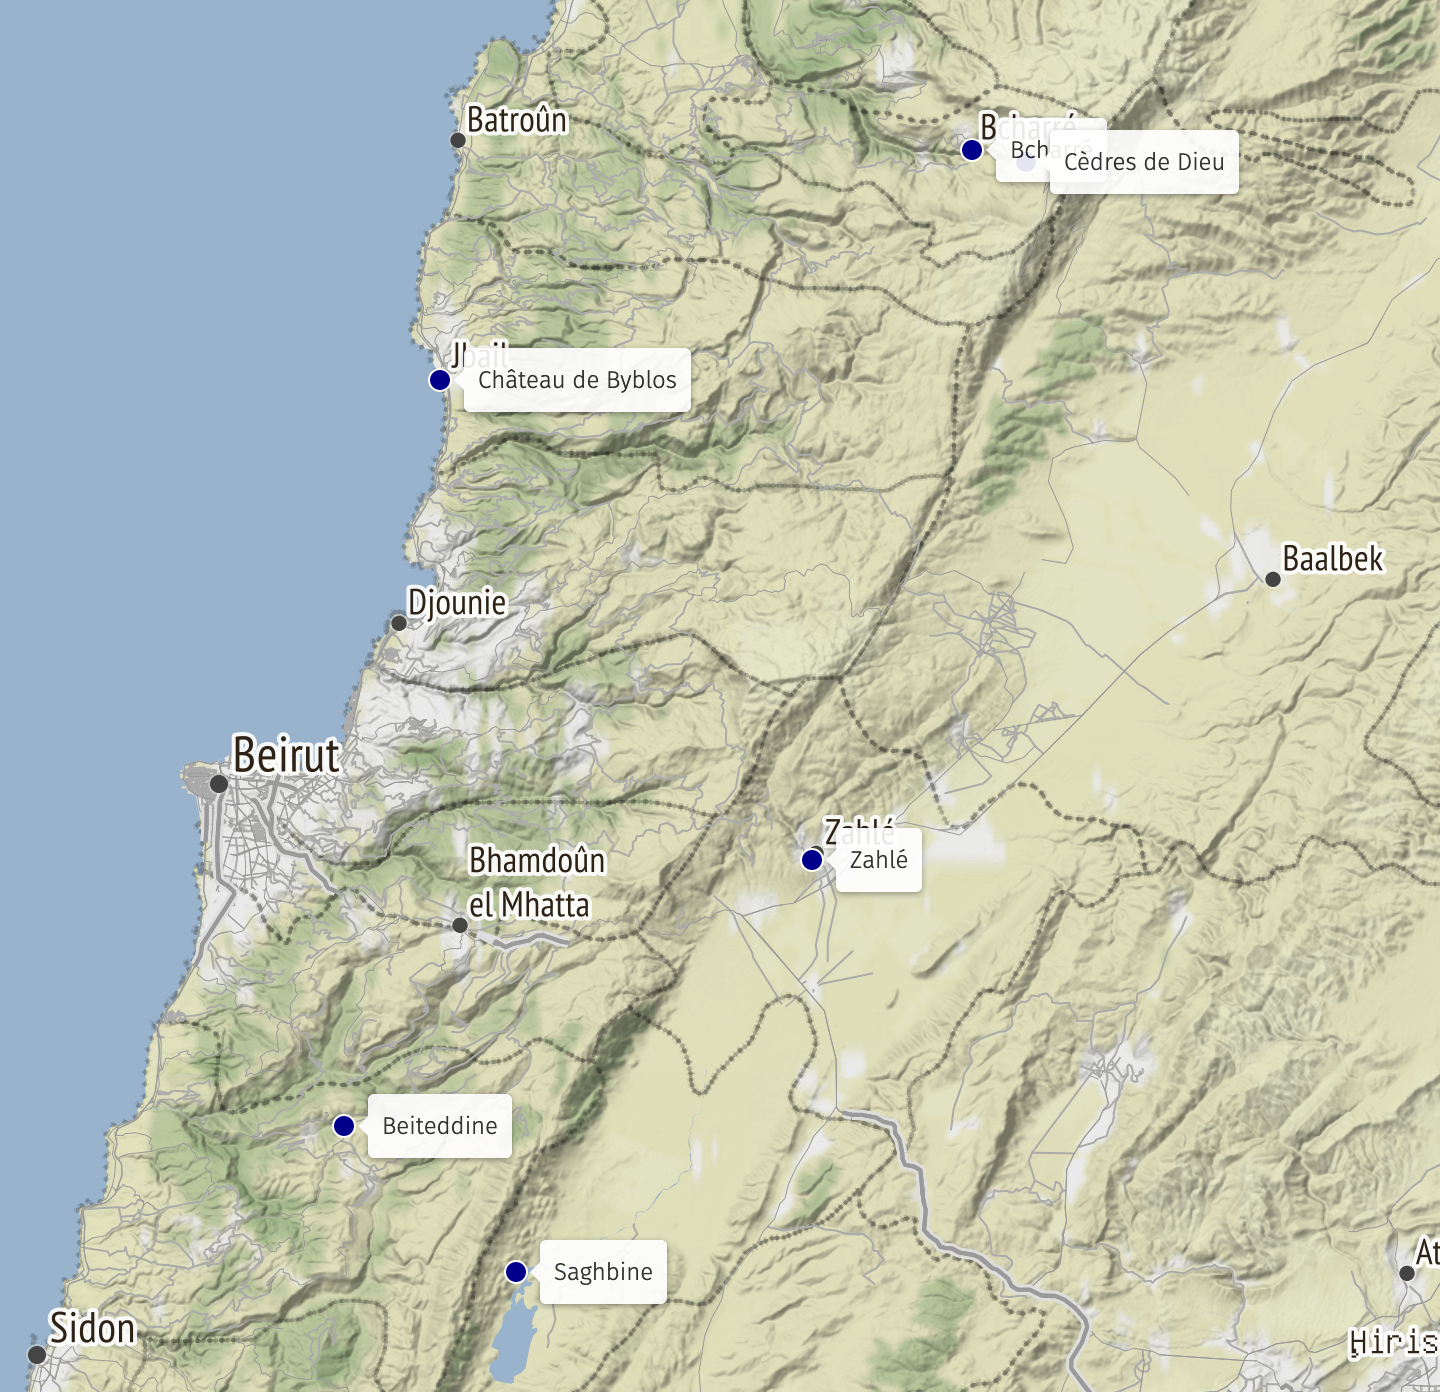
\includegraphics{maps/Liban2.png}
\end{figure}

Dans un climat bien chargé, autant politiquement que météorologiquement
(des pluies battantes et orages en mai pendant plusieurs jours, tous les
libanais nous ont juré n'avoir jamais vu ça...), nous avons tout de même
continué nos explorations diverses. A commencer par les bureaux de vote
! Les élections législatives qui se sont tenues sont les premières
depuis 9 ans. Les gens étaient globalement partagés, entre la motivation
de s'exprimer par les urnes et le côté défaitiste devant la corruption
(on a entendu des promesses d'achats de voix jusqu'à 2000 dollars !) et
les tricheries, qui ont malheureusement bien eu lieu. J'ai choisi mon
camp et je suis allée voter ! (et mon candidat, malgré un score ridicule
dans le village, a bien été élu dans la circonscription !
\textbackslash{}o/). Outre l'omniprésence militaire autour et dans les
bureaux de vote, voir les listes électorales triées par religion fait
toujours son petit effet... Bref, une fois les différents entre
partisans politiques réglés (en gros, une fois que tout le monde s'est
bien foutu sur la tronche), on a pu reprendre le fil de nos excursions.

Nous avons parcouru la vallée de la Bekaa, coincée entre deux chaînes
montagneuses et traversée par le fleuve Litani, retenu par le barrage de
Qaraoun.

\begin{figure}
\centering
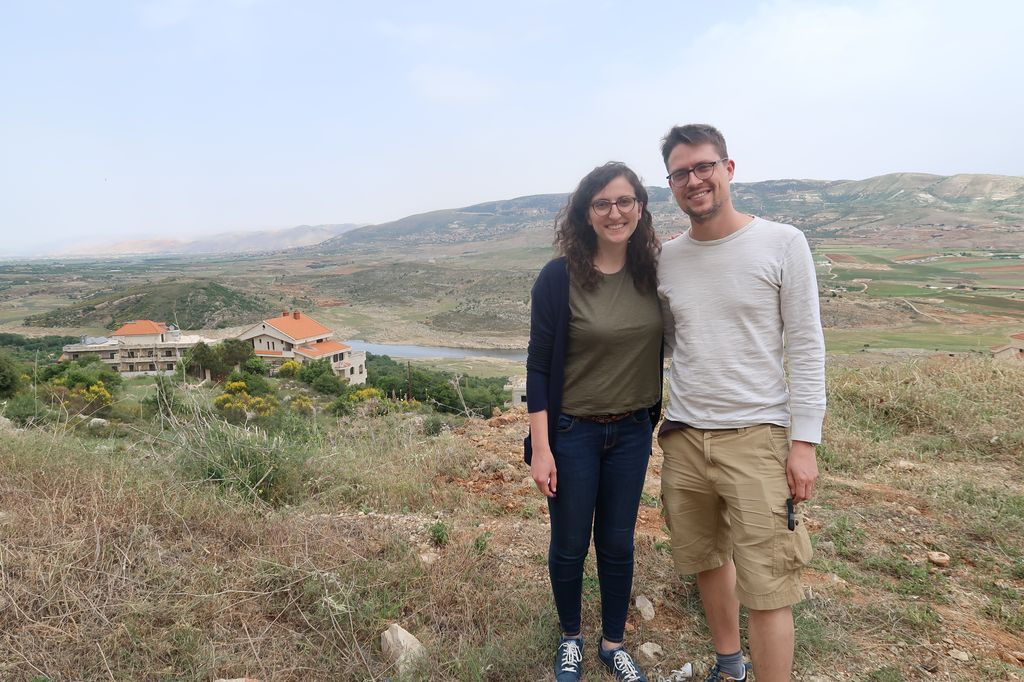
\includegraphics{images/20180517_bekaa.jpg}
\caption{Vallée de la Bekaa après le vote.}
\end{figure}

Un de mes cousins nous a ensuite emmenés vers le palais de Beiteddine,
en passant par la forêt des Cèdres du Chouf (qu'on a pas vraiment vue
-private lebanese joke inside- du fait d'une météo peu clémente dont on
va continuer à se plaindre un peu).

Le palais de Beiteddine a été construit au 19ème siècle pour le grand
émir du Liban. Il est actuellement utilisé comme résidence d'été par le
président de la République, et tous les étés pour le festival de musique
et de danse.

\begin{figure}
\centering
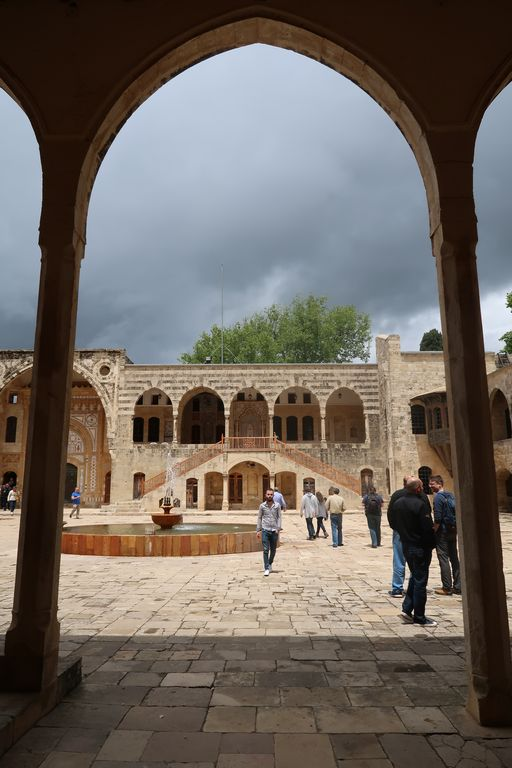
\includegraphics{images/20180517_beiteddine.jpg}
\caption{Le palais, de style ottoman.}
\end{figure}

Zahlé est la capitale du gouvernorat de la Bekaa. Nous avons grimpé les
240 marches de Notre Dame de Zahlé pour admirer la vue panoramique sur
la ville et la vallée. Après un bon taouk (article gastronomique dédié à
venir), nous avons continué nos explorations jusqu'aux caves de Ksara,
où des centaines de tonneaux de vin sont entreposés dans des galeries
datant de l'époque romaine (et où l'on a dégusté le vin produit sur
place).

\begin{figure}
\centering
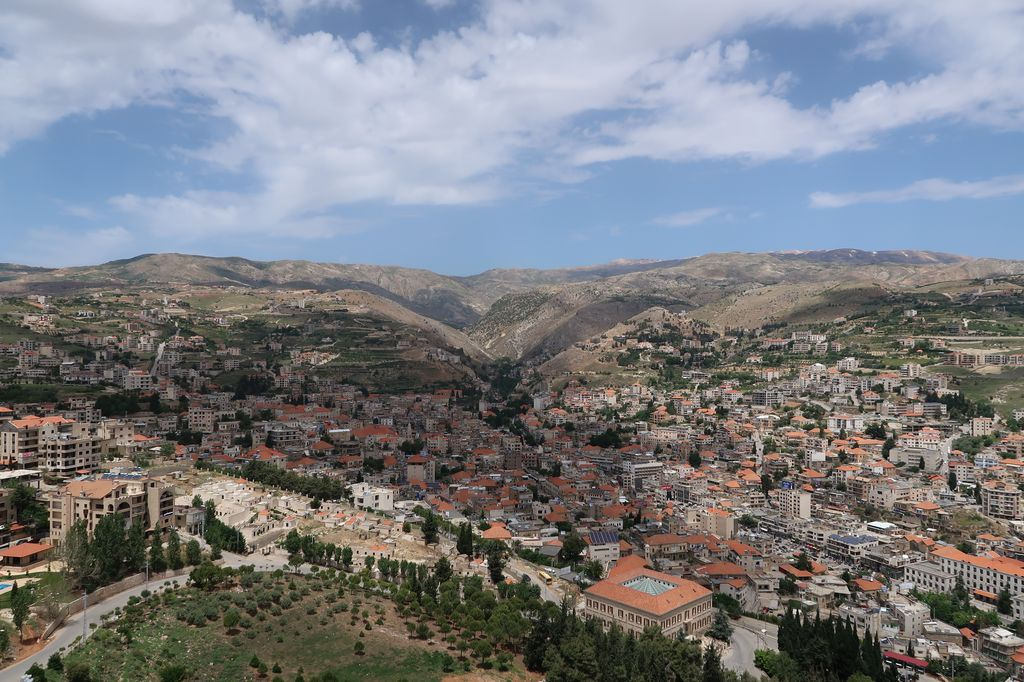
\includegraphics{images/20180517_zahle.jpg}
\caption{Vue panoramique de Zahle.}
\end{figure}

Byblos, que nous avions déjà exploré de nuit la semaine précédente,
mérite le détour de jour pour la visite des vestiges près du port. Le
fort date de l'époque des croisés, mais repose en fait sur les strates
d'occupation plus ancienne (Byblos prétend au titre de ville la plus
vieille du monde). Dans la lumière du jour déclinant, on prend la mesure
de la beauté du site.

\begin{figure}
\centering
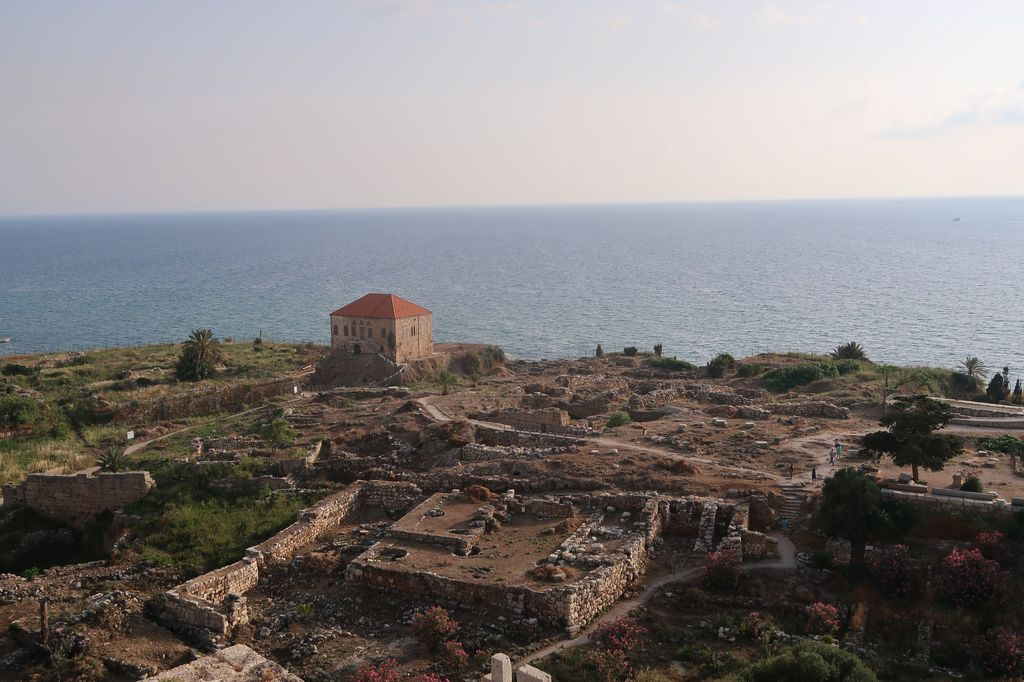
\includegraphics{images/20180517_byblos.jpg}
\caption{Le site de Byblos, au bord de la mer.}
\end{figure}

Premières aventures au volant (et ce n'est pas une mince affaire, vu
l'absence totale de règles de la route "ici, la priorité est au plus
brave", "tu conduis comme tu le sens, et ça marche bien comme ça"), Flo
nous a conduit dans le Nord du pays, jusqu'à une autre forêt de cèdres,
celle de Bcharré. Cette fois nous avons un temps agréable qui nous
permet d'admirer ces colosses parfois millénaires, et dont l'utilisation
du bois est attestée depuis la Mésopotamie... Une balade très agréable,
qui se poursuit à Bcharré où nous visitons le musée de Khalil Gibran
(pour ceux qui ne connaissent pas, lire \emph{Le Prophète} est un must
!), où sont exposées les nombreuses peintures de l'artiste. Cette visite
nous a refait plonger dans ses écrits dont l'extrait suivant nous avait
particulièrement parlé avant notre départ :

\begin{quote}
Me voici prêt à partir, et mon impatience aux voiles déployées attend le
vent. Je ne respirerai qu'une dernière bouffée de cet air calme, je ne
jetterai qu'un dernier regard d'amour en arrière, et alors je serai au
milieu de vous, un navigant parmi les navigants.
\end{quote}

C'est les yeux pleins de ces paysages variés (et les ventres bien
pleins) que la suite se prépare...

\textbf{Bonus demandé par Thibaud : prendre la voiture au Liban.}

Je suis désolé, votre navigateur ne supporte pas les vidéos HTML5 au
format WebM avec VP8 ni au format MP4 avec H.264.

\emph{Elida et Florian}
